\usetikzlibrary{arrows.meta,calc}
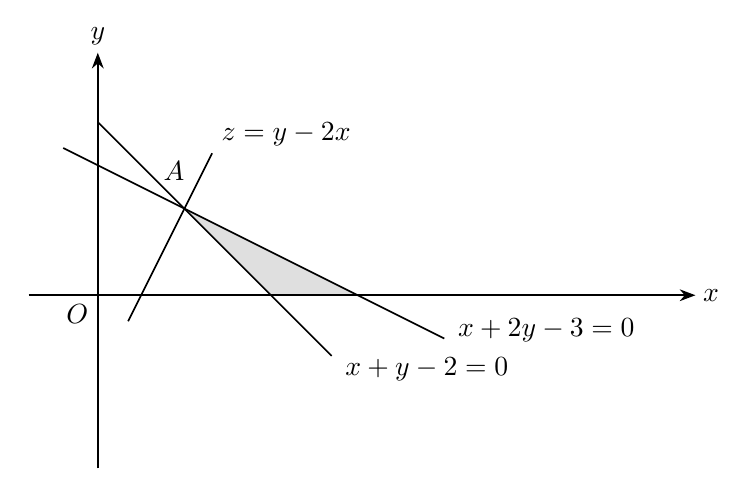
\begin{tikzpicture}[x=1.1cm,y=1.1cm,line width=.6pt,font=\normalsize,>=Stealth]
\fill[gray!25] (1,1)--(2,0)--(3,0)--cycle;
\draw (0,2)--(2.7,-0.7);
\draw (-0.4,1.7)--(4,-0.5);
\draw (0.35,-0.3)--(1.32,1.64);
\draw[->] (-0.8,0)--(6.9,0);
\draw[->] (0,-2.0)--(0,2.8);
\node[anchor=south,inner sep=0pt,yshift=10pt] at (0.88,1.0) {$A$};
\node[anchor=west,inner sep=0pt] at (1.42,1.86) {$z=y-2x$};
\node[anchor=west,inner sep=0pt] at (2.85,-0.85) {$x+y-2=0$};
\node[anchor=west,inner sep=0pt] at (4.15,-0.4) {$x+2y-3=0$};
\node[anchor=north east,inner sep=0pt] at (-0.10,-0.10) {$O$};
\node[anchor=west,inner sep=0pt] at (6.98,0) {$x$};
\node[anchor=south,inner sep=0pt] at (0,2.88) {$y$};
\end{tikzpicture}
